\chapter{TTSP Test and Evaluation}

%-----------------------------------------------------------
% keywords: Test-bed, Tests
%-----------------------------------------------------------
With the purpose of validating the proposed architecture, TTSP was deployed in a WSN test-bed and was subject to a series of test scenarios. These tests intend to evaluate the time synchronization in scenarios ranging from a single node to multiples nodes, from a single-hop network to a multi-hop network, from high precision requirements to much lower precision requirements. Since these tests were designed solely to show how TTSP's synchronization is effective and its features operate, in a qualitative manner, each test was run only once. Being this the case, the obtained results may only be used as a comparison between each test and to validate the effectiveness of the given functionality.\\
%-----------------------------------------------------------
% keywords: Tagus-SensorNet
%-----------------------------------------------------------
Regarding the test-bed, a WSN test-bed, Tagus-SensorNet \cite{conf/icccn/PedrosaMRN08}, allows the unique opportunity to test TTSP in a real deployment scenario, allowing it to experience the intrinsic constraints of a WSN. That is, in Tagus-SensorNet sensor nodes are faced with limited energy resources, communications that can easily be interfered and sensor nodes that can suddenly die or start functioning incorrectly.

\section{Test-bed and Test Scenarios}

\subsection{Tagus-SensorNet}
%-----------------------------------------------------------
% keywords: Tagus-SensorNet
%-----------------------------------------------------------
Tagus-SensorNet sensor nodes, as can be seen in Figure \ref{tsn}, are well dispersed in Taguspark main building.\\

\begin{figure}[!htb]
\begin{center}
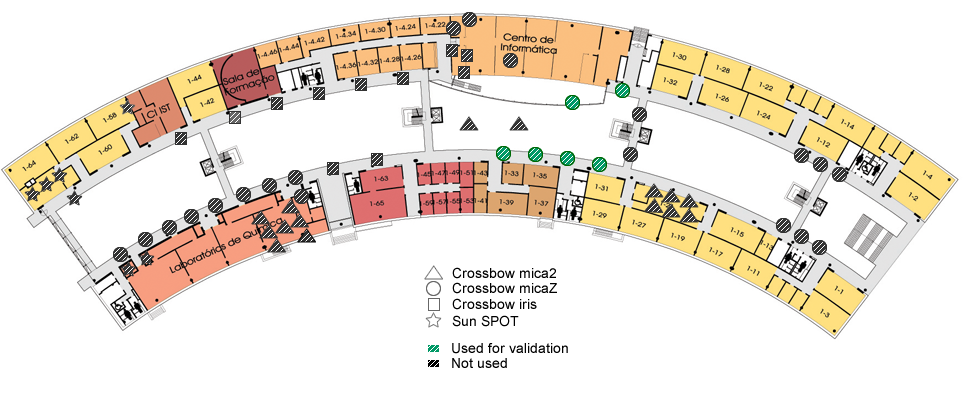
\includegraphics[scale=0.4]{./images/04-tsn-topology.png}
\end{center}
\caption{Tagus-SensorNet current deployment topology.}
\label{tsn}
\end{figure}
%-----------------------------------------------------------
% keywords: 
%-----------------------------------------------------------
The current topology, allows the creation of regions that currently cannot be interconnected, whether it be the physical distance or the heterogeneity of the communication stack, mainly found with the Sun SPOTs and the  Mica family sensor nodes (both Mica2 and MicaZ). Currently, these two family of sensor nodes do not communicate between themselves, although they both have a IEEE 802.14.15 capable radio. The Sun SPOTs run a Java VM while the Mica family sensor nodes run TinyOS.\\
%-----------------------------------------------------------
% keywords: 
%-----------------------------------------------------------
The radio communications that work on the 868/916 MHz and mainly in 2,4 GHz band, face possible interference of other radio technologies that operate on the same band, like IEEE 802.11. This imposes serious communication constraints. But nonetheless, short or long periods of interference are indeed a real
constraint of any WSN.\\
%-----------------------------------------------------------
% keywords: 
%-----------------------------------------------------------
The Mica family sensor nodes are powered by two AAA batteries which also impose serious network lifetime constraints. A sensor node may suddenly die once it's batteries are depleted or stop functioning correctly once the available voltage is lower than the necessary to keep micro-controller, the radio or any other hardware component running correctly.\\
As previously stated, all these constraints, give a unique opportunity for TTSP to be validated correctly, since the real requirements of a WSN are present on this testbed.


\subsection{Test Scenario}
%-----------------------------------------------------------
% keywords: Test Scenario
%-----------------------------------------------------------
The test scenario chosen for this purpose is described in Figure \ref{scenario6}. In this scenario, there are a total of five synchronizing nodes, of which, one node will be declared as the root node, four are to be synchronized with that root node at a given moment in time. One additional node is used as a base-station for continuously collecting the selected metrics from the synchronized nodes and the root node. 

\begin{figure}[!htb]
\begin{center}
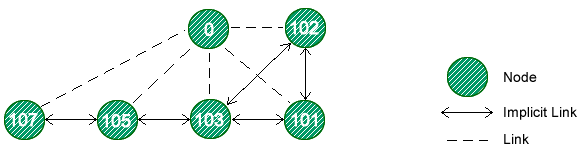
\includegraphics[scale=0.4]{./images/19-ttsp-test_topology.png}
\end{center}
\caption{Six nodes scenario with multi-hop synchronization.}
\label{scenario6}
\end{figure}

Although, most of the used nodes are in the radio coverage of each other, there was the need for a slightly different network topology that could best describe all the physical network topologies that are currently used by other applications in Tagus-SensorNet. For this reason, implicit links were statically configured in each node, which forced the desired logic topology as shown in the previous figure.

\section{Test Application and Methodology}
%-----------------------------------------------------------
% keywords: Test Application
%-----------------------------------------------------------
In order to produce meaningful results from the test-bed, a special test application was developed, which made use of TTSP libraries. This test application acted as an application client by declaring its time precision requirements to TTSP. Every node programmed with this test application was queried by the base-station in order to retrieve the current root node identification and its logical clock time. These values were periodically collected by the base-station, thus it was possible to periodically calculate the time precision error for every node that was synchronized with a root node.

\section{Test Results}
%-----------------------------------------------------------
% keywords: Test Results
%-----------------------------------------------------------
In this section, the processed test results will be presented and briefly discussed. The following indicators have been used across multiple tests:
\begin{itemize}
\item \textit{Precision Error}:  This value, as the name suggests, indicates the current time precision error achieved by a node when synchronized with the root node, measured in time units. This error is obtained from the difference between the local clock of the root node and the logical clock of the synchronizing node, and it is only relevant once this node declared itself synchronized with the root.
\item \textit{Synchronization Period}: This value indicates the current synchronization period being advertised by the root node to the synchronizing nodes. As explained in the previous chapter, the values that this indicator reports are deeply influenced by the current time precision error achieved with the synchronizing nodes.
\end{itemize}

\clearpage

\subsection{Single-hop/-node Synchronization With High Precision Requirements}
%-----------------------------------------------------------
% keywords: 
%-----------------------------------------------------------
A single-hop with only one node to synchronize with the root node is the basic scenario where TTSP can be used. This scenario was chosen in order to evaluate the efficiency and effectiveness of the TTSP's response which is directly influenced by the time precision error monitored from its synchronizing nodes, thus the number of synchronizing nodes is relevant for the evaluation of TTSP. For this first scenario a high precision requirement of a maximum time precision error of 10 ms was chosen. The results of this scenario can be found in Figure \ref{10ms2nodes}.

\begin{figure}[!htb]
\begin{center}
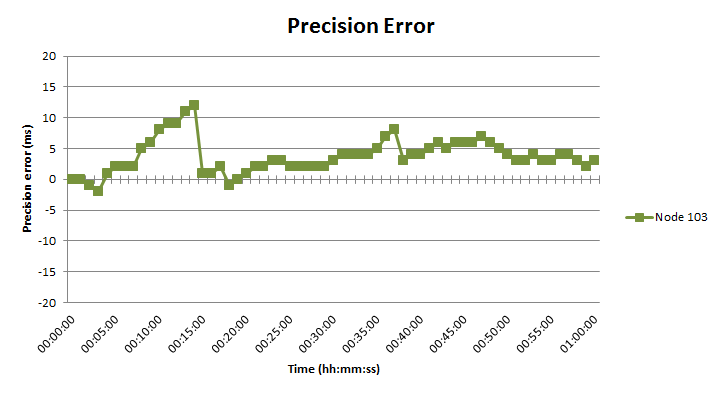
\includegraphics[scale=0.4]{./images/09-ttsp-10ms2nodes-error.png}
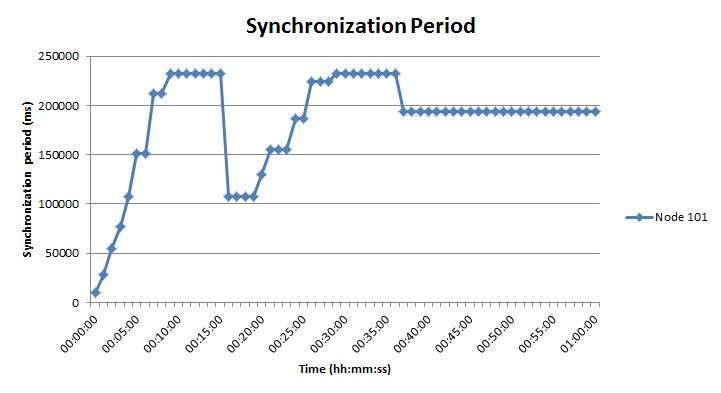
\includegraphics[scale=0.4]{./images/10-ttsp-10ms2nodes-period.png}
\end{center}
\caption{Single-hop/-node synchronization results with a precision error requirement of 10 ms.}
\label{10ms2nodes}
\end{figure}

The results indicate, that for a single-hop synchronization of a single node, the synchronization period converges to an approximated value of 194 seconds while ensuring that the time precision error is below the required value.

\subsection{Single-hop/-node Synchronization With Low Precision Requirements}
%-----------------------------------------------------------
% keywords:
%-----------------------------------------------------------
This scenario resembles almost everything with the previous one, except that the requested maximum time precision error is higher, thus a lower precision requirement which will also significantly influence the efficiency and effectiveness of TTSP's response. For the previous scenario of a single node a lower precision requirement of only 50 ms was required to TTSP. The obtained results are shown in Figure \ref{50ms2nodes}.

\begin{figure}[!htb]
\begin{center}
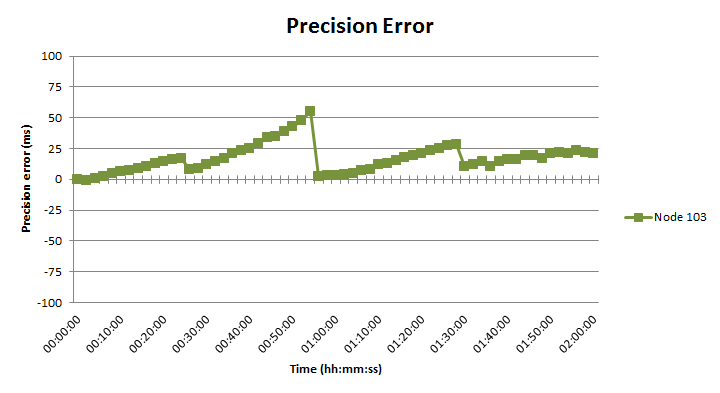
\includegraphics[scale=0.4]{./images/20-ttsp-50ms2nodes-error.png}
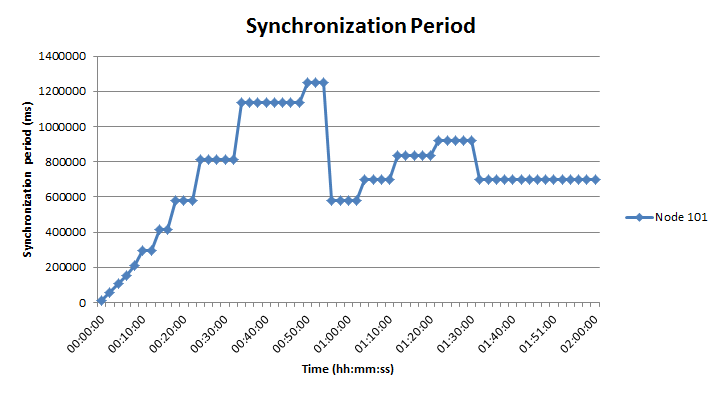
\includegraphics[scale=0.4]{./images/21-ttsp-50ms2nodes-period.png}
\end{center}
\caption{Single-hop/-node synchronization results with a error precision requirement of 50 ms.}
\label{50ms2nodes}
\end{figure}

The results show that for a time precision error lower than 50 ms, the synchronization period converges to an approximated value of 11 minutes and 37 seconds, which is entirely justified by the more relaxed precision requirements. One also needs to take into consideration the increased amount of time needed to converge to a synchronization period when compared with the results of the past scenario.

\subsection{Multi-hop/node Synchronization With High Precision Requirements}
%-----------------------------------------------------------
% keywords: multi-hop/node synchronization with high precision requirements
%-----------------------------------------------------------
In this scenario, multiple nodes are used with multi-hop being used by some of these in order for synchronization to be realized. This scenario is described in Figure \ref{scenario6}. For this scenario, it was requested from TTSP that the maximum precision error did not exceed the 10 ms. The obtained results in Figure \ref{10ms6nodes}.

\begin{figure}[!htb]
\begin{center}
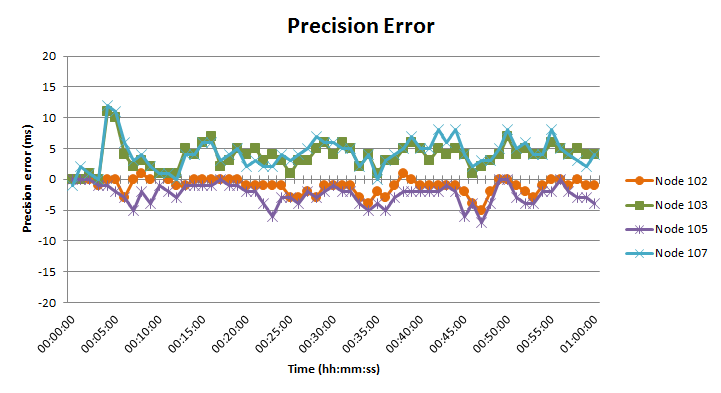
\includegraphics[scale=0.4]{./images/11-ttsp-10ms6nodes-error.png}
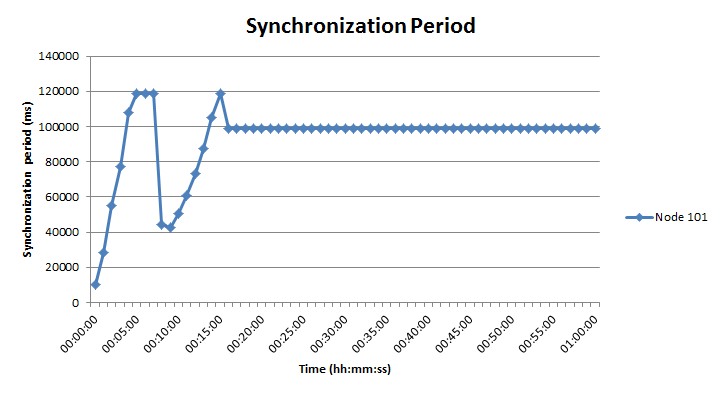
\includegraphics[scale=0.4]{./images/12-ttsp-10ms6nodes-period.png}
\end{center}
\caption{Time precision error with a precision request of 10 ms and using 6 nodes.}
\label{10ms6nodes}
\end{figure}

The results clearly show that for an increased number of synchronizing nodes, the synchronization period converges much faster, almost twice as fast when synchronizing only one node as shown in the first experiment results in Figure \ref{10ms2nodes} with the same time precision requirements. This is justified by the increased number of nodes, which allow for a faster synchronization period convergence, since multiple feedbacks are used to actuate on the synchronization period. Even though the root node filters neighbours feedback by the sequence number of the synchronization round, it also takes into account the total number of acceptable and unacceptable feedback received to adjust the synchronization period.
This awareness allows TTSP to converge the synchronization period faster. This fast convergence is clearly justified by the increased number of synchronizing nodes. Although, a fast convergence of the synchronization period was observed, the final achieved synchronization period was almost half as what was achieved with only one node. This can also be justified by the number of synchronizing nodes, more specifically the probability of existence of synchronizing nodes with clock drifts completely different than the root node, which will result in higher absolute precision errors, thus forcing a lower synchronization period for the network-wide synchronization.

\clearpage

\subsection{Multi-hop/-node Synchronization With Low Precision Requirements}
%-----------------------------------------------------------
% keywords: multi-hop/node synchronization with low precision requirements
%-----------------------------------------------------------
For this experiment, the previous scenario was used, the only changed parameter as like the experiment with the single-node, was the maximum time precision error allowed in the network. Thus, the maximum tolerable precision error was increased to 50 ms. The obtained results can be seen in Figure \ref{50ms6nodes}.

\begin{figure}[!htb]
\begin{center}
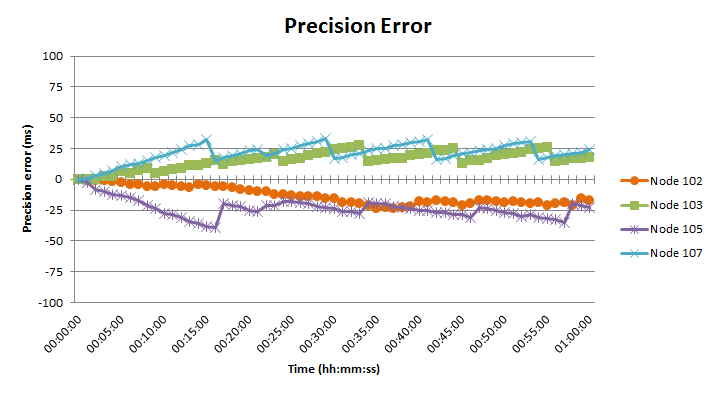
\includegraphics[scale=0.4]{./images/23-ttsp-50ms6nodes-error.png}
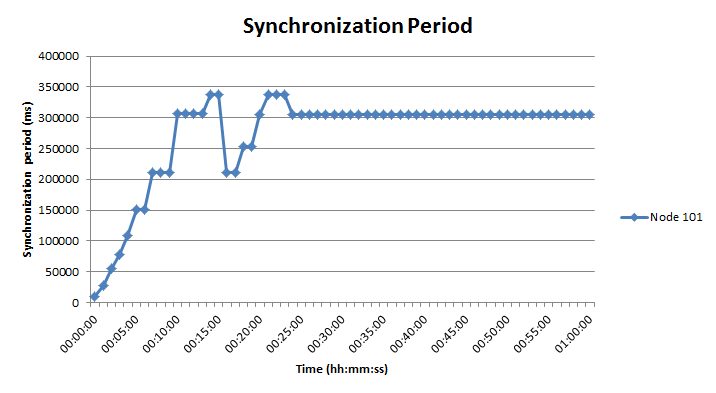
\includegraphics[scale=0.4]{./images/22-ttsp-50ms6nodes-period.png}
\end{center}
\caption{Time precision error with a precision request of 50 ms and using 6 nodes.}
\label{50ms6nodes}
\end{figure}

It is possible to conclude from these results, that the relaxation of the requirements tend to have the same effect as in the case of a single node, that is, a slower synchronization convergence but a higher synchronization period. One can extend this observation, by stating that the synchronization period converged at 24 minutes since the beginning of this experiment, eight more minutes than the needed in the previous experiment with a requirement of a time precision error below of 10 ms, showing that the difference is not that higher as with the experiment with the single-node.

\clearpage

\subsection{Fast Synchronization Mechanism}
%-----------------------------------------------------------
% keywords: fast synchronization mechanism
%-----------------------------------------------------------
The objective with this experiment is to assess the fast synchronization mechanism that is triggered when for example a node joins the network for a first time after the synchronization period has already converged or the re-election mechanism has been triggered and the information of the new root is being propagated throughout the network. In this typical situation the new node will have to collect four synchronization points from a root node or a neighbouring node. Without the use of this mechanism, the new node would have to wait for four times the current synchronization period in order to get synchronized with the root node. The fast mechanism basically detects new nodes and triggers a consecutive broadcast of four samples in order for the new node to get quickly synchronized with the root node. In Figure \ref{fastsync} it is possible to verify the obtained results with the use of this mechanism, it is important to detail that the new node (node 107) was turned on at exactly 40 minutes since the beginning of the test.

\begin{figure}[!htb]
\begin{center}
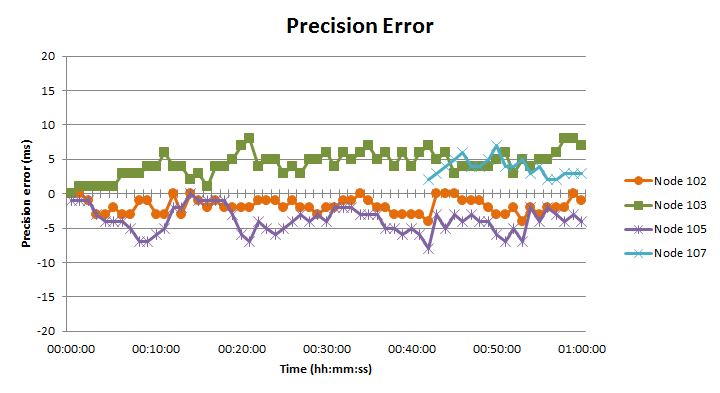
\includegraphics[scale=0.4]{./images/15-ttsp-10ms6nodes-fastsync-error.png}
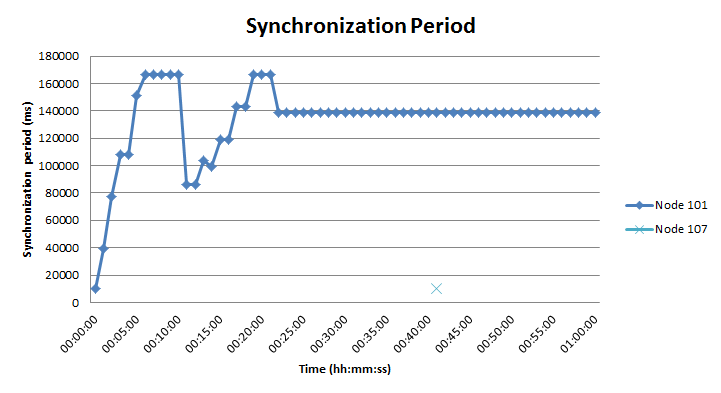
\includegraphics[scale=0.4]{./images/16-ttsp-10ms6nodes-fastsync-period.png}
\end{center}
\caption{Fast synchronization mechanism.}
\label{fastsync}
\end{figure}

Regarding this case, after the new node was turned on, and past the time duration of three times the initial synchronization period without hearing a synchronization broadcast, it declares itself root, in this case after 30 seconds, since the default initial synchronization period was set to 10 seconds. It could happen that the new node could hear a synchronization broadcast from one of its neighbours, which did not happened in this specific case. In those situations however, the new node would have discard the synchronization point by looking at the synchronization period which is clearly different from the initial synchronization period. Once the new node elects himself, he starts to broadcast its local clock with a period of 10 seconds. The first broadcast is heard by its neighbouring nodes which are already synchronized with root node with an identification lower than the new node. This triggers the fast synchronization mechanism in the neighbouring nodes, which leads the new node to be aware of the actual root node and became synchronized with it. 

\clearpage

\subsection{Re-election Mechanism}
%-----------------------------------------------------------
% keywords: re-election mechanism
%-----------------------------------------------------------
In this experiment, the objective is to assess the re-election mechanism which must be executed once the current root node ceases to broadcast its local clock. The used scenario is the same as the one used with the multiple nodes and existence of multi-hop synchronization. The experiment is composed of a initial period where all synchronizing nodes will eventually synchronize with an elected root node, and consequently that root node will be remotely turned off, ceasing to broadcast its local clock. The remaining nodes, must continue to be synchronized among themselves, for that, the re-elections mechanism will be triggered and a new root node elected. The results of this experiment can be seen in Figure \ref{reelection}.

\begin{figure}[!htb]
\begin{center}
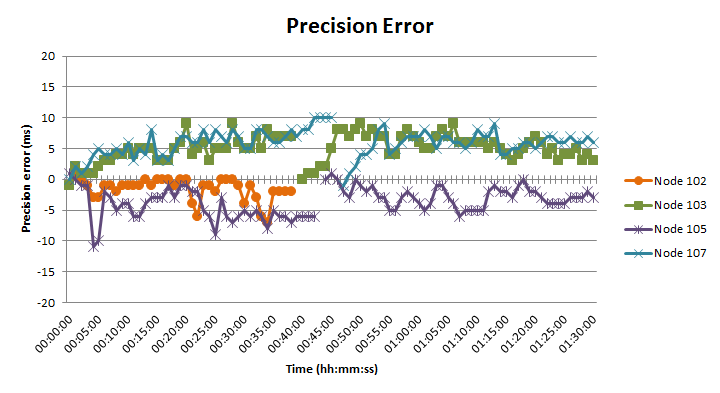
\includegraphics[scale=0.4]{./images/13-ttsp-10ms6nodes-reelection-error.png}
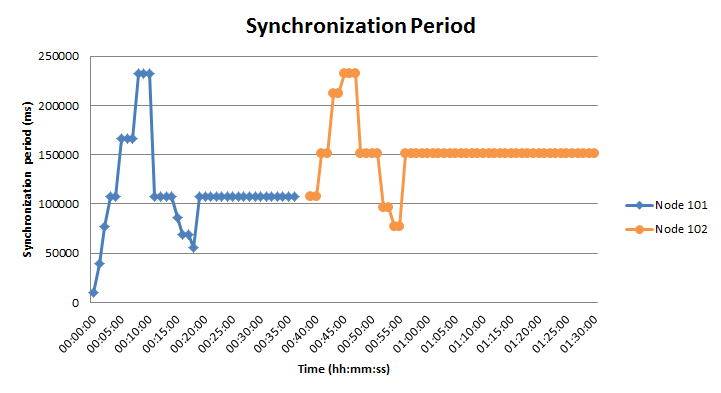
\includegraphics[scale=0.4]{./images/14-ttsp-10ms6nodes-reelection-period.png}
\end{center}
\caption{Re-election mechanism.}
\label{reelection}
\end{figure}

The results are clear enough to tell that the new root node is elected, the remaining node with the lower identification. This process is triggered on each node after a root silence of three times the current synchronization period. In this case, 312 seconds after the first root node broadcasted its last local clock. After the re-election process is triggered,  the recent elected node continues with the same synchronization period than its predecessor, but becomes aware of the current low absolute precision error gathered from the synchronizing nodes and adaptively adjusts the synchronization period to a best suitable one.

\clearpage

\subsection{Multi-hop/-node Synchronization with High Requirements Extended Duration}
%-----------------------------------------------------------
% keywords: 
%-----------------------------------------------------------
This experiments objective was different from the previous ones. The sole purpose of this experiment is to assess the effectiveness of TTSP synchronization over a longer period. This experiment was necessary due to the stringent need of keeping the maximum precision error lower than the requested and keep the synchronization period stable over a longer period. A twenty-four hour experiment of TTSP on Tagus-SensorNet is acceptable for this objective and the obtained results can be seen in Figure \ref{24h}.

\begin{figure}[!htb]
\begin{center}
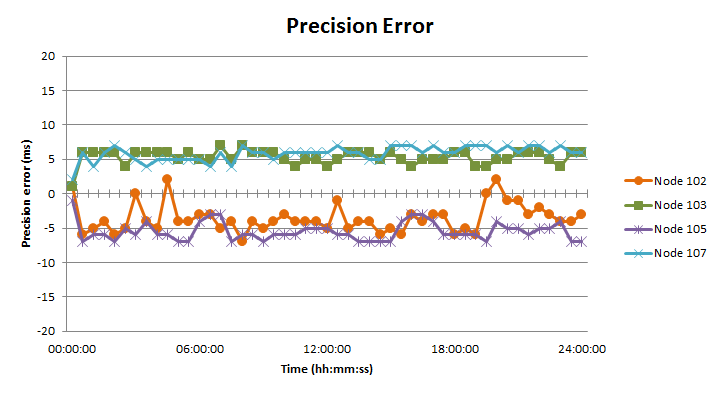
\includegraphics[scale=0.4]{./images/17-ttsp-10ms5nodes-error.png}
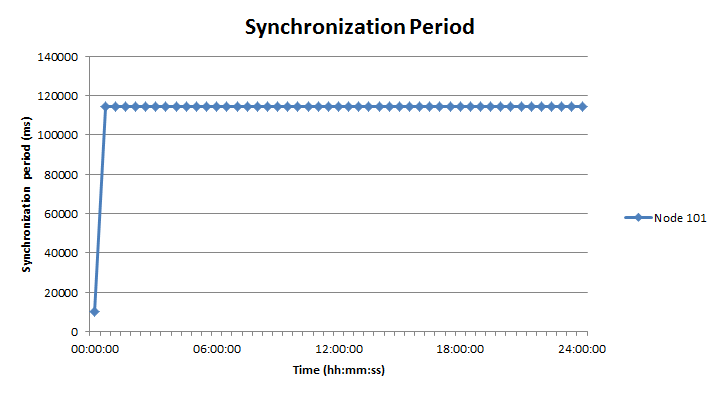
\includegraphics[scale=0.4]{./images/18-ttsp-10ms5nodes-period.png}
\end{center}
\caption{Time precision error with a precision request of 10 ms and using 5 nodes.}
\label{24h}
\end{figure}

As predicted, without any changes involving the root node, the time precision error on all nodes in the network keeps below the maximum allowed threshold and the synchronization period keeps unchanged. One can conclude, that the requirements were fulfilled during this twenty-four hour period, and the time synchronization protocol operated stable under normal circumstances that Tagus-SensorNet is daily subject to. The interference from closely wireless networks such as the campus 802.11 infrastructure network (which covers the whole main building) did not significantly influenced TTSPs effectiveness as all nodes kept synchronized with a precision error lower than the requested throughout the twenty-four hour period.